\documentclass[aspectratio=169]{beamer}

\usetheme{Madrid}
\usecolortheme{seahorse}
\usefonttheme{professionalfonts}

\usepackage{listings}
\usepackage{xcolor}
\usepackage{tikz}
\usepackage{booktabs}
\usepackage{hyperref}
\usepackage{textcomp}
\usepackage{microtype}

\definecolor{codebg}{HTML}{1E1E2E}
\definecolor{codegreen}{HTML}{A6E3A1}
\definecolor{codeblue}{HTML}{89DCEB}
\definecolor{codeyellow}{HTML}{F9E2AF}
\definecolor{codegray}{HTML}{6C7086}
\definecolor{codepurple}{HTML}{CBA6F7}
\definecolor{codeorange}{HTML}{FAB387}
\definecolor{codewhite}{HTML}{CDD6F4}

\lstdefinestyle{clang}{
  backgroundcolor=\color{codebg},
  basicstyle=\ttfamily\footnotesize\color{codewhite},
  keywordstyle=\color{codepurple}\bfseries,
  commentstyle=\color{codegray}\itshape,
  stringstyle=\color{codegreen},
  numberstyle=\tiny\color{codegray},
  numbers=left, numbersep=6pt,
  breaklines=true, frame=single,
  rulecolor=\color{codeblue},
  language=C,
  tabsize=4
}

\title[MyOS Chapter 7]{\textbf{MyOS Chapter 7: Multitasking (Round-Robin Scheduler)}}
\subtitle{Background tasks + timer ticks + scheduler observability}
\author{MyOS Project}
\date{March 2026}
\institute{x86 Protected Mode Kernel Engineering}

\newcommand{\concept}[2]{%
  \begin{block}{#1}\smallskip #2\smallskip\end{block}\vspace{5pt}}

\newcommand{\warn}[1]{%
  \begin{alertblock}{Important}\smallskip #1\smallskip\end{alertblock}\vspace{5pt}}

\begin{document}

\begin{frame}
  \titlepage
\end{frame}

\begin{frame}{Learning objectives}
  \begin{itemize}
    \item Understand preemptive scheduling trigger via hardware timer IRQ
    \item Implement a round-robin scheduler for multiple background tasks
    \item Add shell controls to start/list/stop background jobs
    \item Keep OS time ticking continuously from PIT interrupts
  \end{itemize}
\end{frame}

\begin{frame}{What was implemented}
  \begin{itemize}
    \item PIT timer configured at 100 Hz (IRQ0)
    \item IRQ handler dispatches both timer (IRQ0) and keyboard (IRQ1)
    \item Round-robin scheduler with runtime-created named background tasks
    \item Background-task shell commands: \texttt{bg run/list/stop} for arbitrary task names
    \item Tick, uptime, and software clock APIs for runtime visibility
  \end{itemize}
\end{frame}

\begin{frame}{System flow: interrupt to task execution}
\begin{center}
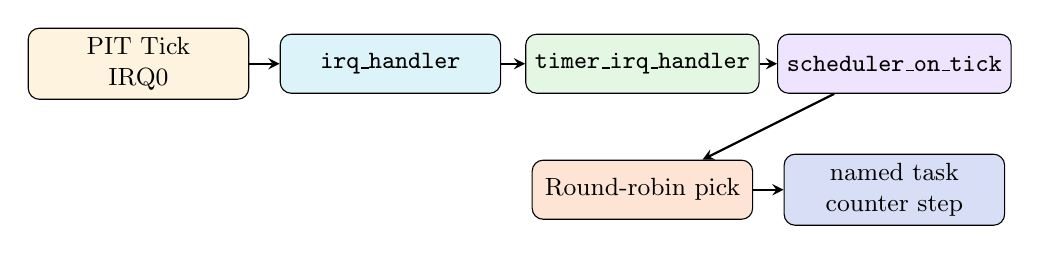
\begin{tikzpicture}[
  box/.style={rectangle,draw,rounded corners=4pt,
    minimum width=2.8cm,minimum height=0.75cm,
    align=center,font=\small},
  arr/.style={->,thick,>=stealth}]

  \node[box,fill=codeyellow!40] (pit) at (0,0) {PIT Tick\\IRQ0};
  \node[box,fill=codeblue!30] (irq) at (3.2,0) {\texttt{irq\_handler}};
  \node[box,fill=codegreen!30] (timer) at (6.4,0) {\texttt{timer\_irq\_handler}};
  \node[box,fill=codepurple!30] (sched) at (9.6,0) {\texttt{scheduler\_on\_tick}};

  \node[box,fill=codeorange!35] (rr) at (6.4,-1.6) {Round-robin pick};
  \node[box,fill=codewhite!80] (run) at (9.6,-1.6) {named task\\counter step};

  \draw[arr] (pit) -- (irq);
  \draw[arr] (irq) -- (timer);
  \draw[arr] (timer) -- (sched);
  \draw[arr] (sched) -- (rr);
  \draw[arr] (rr) -- (run);
\end{tikzpicture}
\end{center}
\end{frame}

\begin{frame}[fragile]{Timer core (100 Hz PIT)}
\begin{lstlisting}[style=clang]
void timer_init(uint32_t hz) {
    tick_hz = hz;
    divisor = 1193180 / tick_hz;

    outb(0x43, 0x36);
    outb(0x40, divisor & 0xFF);
    outb(0x40, (divisor >> 8) & 0xFF);
}

void timer_irq_handler() {
    timer_ticks++;
    scheduler_on_tick(timer_ticks);
    ... // uptime and clock update
}
\end{lstlisting}
\concept{Why 100 Hz?}{
  10 ms scheduling quantum: responsive enough for demonstration, simple for arithmetic.
}
\end{frame}

\begin{frame}[fragile]{IRQ integration changes}
\begin{lstlisting}[style=clang]
void irq_handler(registers_t* regs) {
    if (regs->int_no == 32) {
        timer_irq_handler();
    }
    if (regs->int_no == 33) {
        keyboard_irq_handler();
    }
    ... // PIC EOI
}
\end{lstlisting}
\begin{itemize}
  \item PIC mask changed to allow IRQ0 and IRQ1
  \item Timer and keyboard now co-exist under same interrupt framework
\end{itemize}
\end{frame}

\begin{frame}[fragile]{Round-robin scheduler design}
\begin{lstlisting}[style=clang]
for (tries = 0; tries < SCHED_MAX_TASKS; tries++) {
    rr_last_index = (rr_last_index + 1) % SCHED_MAX_TASKS;
    if (!task_table[rr_last_index].active) continue;

    task->runs++;
    task->last_tick = tick_count;
    task->step(task);    // increments task counter
    break;
}
\end{lstlisting}
\concept{Round-robin property}{
  Every active task gets fair turn in cyclic order, one task per timer tick.
}
\end{frame}

\begin{frame}{Background task model used}
  \begin{itemize}
    \item Any task name can be created (e.g. \texttt{alpha}, \texttt{render}, \texttt{netrx})
    \item Each task maintains a \texttt{counter} incremented on each scheduled run
    \item \texttt{runs} shows total schedule events, \texttt{last\_tick} shows most recent tick
  \end{itemize}
  \concept{Purpose of demo tasks}{
    Keep work deterministic and lightweight while proving fairness and concurrent progress.
  }
\end{frame}

\begin{frame}{Shell commands for background execution}
  \small
  \begin{tabular}{@{}p{3.2cm}p{8.8cm}@{}}
    \toprule
    \textbf{Command} & \textbf{Behavior} \\
    \midrule
    \texttt{bg run alpha} & starts a task named \texttt{alpha} and assigns task id \\
    \texttt{bg run worker1} & starts any other named counting background task \\
    \texttt{bg run all} & starts default demo set: \texttt{task1}, \texttt{task2}, \texttt{task3} \\
    \texttt{bg list} & shows id, name, run count, counter value, and last tick \\
    \texttt{bg stop 2} & stops task with id 2 \\
    \texttt{bg stop alpha} & stops task by name \\
    \texttt{bg stop all} & stops every background task \\
    \bottomrule
  \end{tabular}
\end{frame}

\begin{frame}{Are these tasks real?}
  \begin{itemize}
    \item Yes: task scheduling is driven by real kernel timer IRQ0 events
    \item Yes: task state is stored in kernel memory and updated by scheduler ticks
    \item The environment is QEMU-emulated hardware, but scheduling logic is native OS code
  \end{itemize}
  \concept{Interpretation}{
    This is genuine kernel multitasking behavior at the scheduler layer,
    before full CPU register context-switch implementation.
  }
\end{frame}

\begin{frame}{Keeping time ticking in OS}
  \begin{itemize}
    \item Timer interrupt increments global tick counter continuously
    \item Every \texttt{Hz} ticks, OS uptime seconds increase
    \item Software clock (HH:MM:SS) advances each second
    \item Shell commands: \texttt{ticks}, \texttt{uptime}, \texttt{time}, \texttt{set time HH:MM:SS}
  \end{itemize}
\end{frame}

\begin{frame}{Keyword glossary}
  \small
  \begin{tabular}{@{}p{3.0cm}p{9.0cm}@{}}
    \toprule
    \textbf{Keyword} & \textbf{Meaning} \\
    \midrule
    \texttt{PIT} & Programmable Interval Timer chip generating periodic IRQ0 ticks. \\
    \texttt{IRQ0} & Timer interrupt line used as scheduler heartbeat. \\
    \texttt{Round-robin} & Cyclic scheduling policy giving each task a fair turn. \\
    \texttt{Quantum} & Time slice available before scheduler moves to next task. \\
    \texttt{Background task} & Task executed by scheduler without blocking shell input loop. \\
    \texttt{Tick} & Single timer interrupt event; base time unit in scheduler. \\
    \texttt{Uptime} & Total running time since boot, derived from ticks. \\
    \bottomrule
  \end{tabular}
\end{frame}

\begin{frame}{Core module changes}
  \small
  \begin{tabular}{@{}p{2.7cm}p{9.3cm}@{}}
    \toprule
    \textbf{Module} & \textbf{Change} \\
    \midrule
    \texttt{timer.c/h} & New PIT setup, tick counting, uptime, and software clock APIs \\
    \texttt{scheduler.c/h} & New task table, round-robin engine, start/stop/list interfaces \\
    \texttt{isr.c} & IRQ0 dispatch added before keyboard IRQ1 handling \\
    \texttt{idt.c} & PIC mask updated to enable both timer and keyboard lines \\
    \texttt{kernel.c} & Added \texttt{scheduler\_init()} and \texttt{timer\_init(100)} in boot path \\
    \texttt{shell.c} & Added background-task and time-tick shell commands \\
    \bottomrule
  \end{tabular}
\end{frame}

\begin{frame}{Demonstration sequence}
  \begin{enumerate}
    \item Boot and run \texttt{ticks} twice; value must increase
    \item Run \texttt{bg run alpha} and \texttt{bg run render}
    \item Run \texttt{bg list} repeatedly; both \texttt{runs} and \texttt{counter} must increase
    \item Run \texttt{uptime}; verify steady growth
    \item Stop one task with \texttt{bg stop alpha}
    \item Run \texttt{bg list} to verify only remaining tasks advance
  \end{enumerate}
\end{frame}

\begin{frame}{Limits and next evolution}
  \begin{itemize}
    \item Current scheduler runs task \texttt{step()} functions, not full CPU-context switching
    \item No per-task stack/register save-restore yet
    \item Next step: true task contexts, stack switching, and preemptive task frames
  \end{itemize}
  \warn{This stage is a strong multitasking foundation and a correct bridge to full context-switching kernels.}
\end{frame}

\begin{frame}{Outcome}
  \begin{itemize}
    \item MyOS now has a working round-robin scheduler heartbeat
    \item Background tasks are controllable from shell in real time
    \item Timer-driven OS clock and uptime are continuously maintained
    \item Kernel architecture is now ready for advanced task context switching
  \end{itemize}
  \vspace{8pt}
  \begin{center}
    \Large \textbf{Chapter 7 unlocks real-time kernel multitasking behavior.}
  \end{center}
\end{frame}

\end{document}
